% !TEX root = ../main.tex

\chapter{绪论}
\label{cha:intro}


\section{研究背景与意义}
\label{sec:meaning}

% 挑战 ---工业系统是基础设施并且高复杂性高耦合,一旦发生故障后果严重
工业系统是国民经济和国家安全的重要基础,在军事、交通和制造业等领域得到广泛应用。然而工业系统普遍集成度高、耦合关系复杂,任何零部件出现故障都可能导致重大损失。比如1986年骇人听闻的美国挑战者号空难,航天飞机发射73秒后解体,飞行员全部遇难\cite{united1986report};1998年发生在德国埃舍德的高速列车重大事故导致101人死亡\cite{oestern2000facts}。随着工业科技的进步,工业系统集成度越来越高,耦合关系越来越复杂。比如典型的汽车有大约2千功能部件、3万个零件和1千万行软件代码\cite{tsui2015prognostics}。如何保障日趋复杂的工业系统可靠、安全、可持续的运行面临严峻挑战。
% 1986年,美国挑战者号空难,The failure was caused by the fact that O-ring seals used in the joint were not designed to handle the unusually cold conditions that existed at this launch.The seals' failure caused a breach in the SRB joint, allowing pressurized burning gas from within the solid rocket motor to reach the outside and impinge upon the adjacent SRB aft field joint attachment hardware and external fuel tank. 
%(https://en.wikipedia.org/wiki/Space_Shuttle_Challenger_disaster)

% 挑战 --- 传统维修体制与维修高开支之间的矛盾
维修技术是保障工业系统安全运行的主要手段\cite{jardine2006review}。早期的维修技术主要为失效后维修。为了满足日益增长的安全性需求,维修体制逐渐向计划维修体制过渡,即定期对系统进行预防性的检查、保养和维修。然而劳动密集型的计划维修体制高度依赖专家和技术人员的领域知识,大多通过感觉器官进行检修,存在维修量大、工作强度高、效率低下等问题。随着系统复杂性不断提升,维修成本不断攀升以至于已经成为很多工业公司的主要支出\cite{peng2010current},各企业的维修费用通常可占总支出的15-70\%\cite{王凌2007维修决策模型和方法的理论与应用研究}。安全性和维修成本之间的矛盾亟待缓解。

% 挑战 --- 工业转型对工业系统安全性的要求越来越高。
在信息化浪潮下物联网技术日渐成熟,融合信息技术和物理系统技术的以“智能制造”为核心的第四次工业革命拉开序幕。各国纷纷制定政策以做好准备迎接工业转型的挑战与机遇。德国为维护其在工业领域的霸主地位,率先提出“工业4.0”概念并制定一系列相关战略\cite{kagermann2013recommendations}。美国为保障未来的全球竞争力颁布了《先进制造业合作伙伴》战略\cite{advanced2012capturing}。我国作为工业大国,政府颁布了以实现制造强国为战略目标的《中国制造2025》政策\cite{周济2015智能制造——“中国制造}。一方面,随着工业转型,更智能化的工业系统在国家基础建设和发展进程中将扮演更重要的角色,安全问题不容忽视。另一方面,“工业4.0”的转型升级使大量工业数据得到有效的采集、传输和存储,来自麦肯锡全球研究所的技术报告直接指出——大数据技术将作为工业发展的基础渗透于工业生产全过程\cite{manyika2011big},丰富的数据资源蕴含着巨大价值,为利用先进机器学习和数据挖掘技术助力工业转型提供充足资源。
%随着工业转型,更智能化的工业系统在国家基础建设和发展进程中将扮演更重要的角色,安全问题不容忽视,《中国制造2025》中“质量为先”的基本方针更是充分体现了安全问题在工业转型中的重要性。

% 机遇 ---- 传感器技术的成熟,工业大数据是丰富的资源,维修体制升级
%传感器技术的成熟使大量工业数据得到有效的采集、传输和存储。来自麦肯锡全球研究所的技术报告直接指出——大数据技术将作为工业发展的基础渗透于工业生产全过程\cite{manyika2011big}。
抓住工业大数据带来的新机遇,维修技术逐渐向更高效的视情维修(Condition-Based Maintenance,CBM)发展\cite{jardine2006review, peng2010current}。视情维修主要由数据获取、数据处理和维修决策三个步骤组成,基于获取的数据以数据处理为手段挖掘潜在价值实现系统故障诊断和预测,进而作出是否采取维修行为的决策,可在很大程度上减少计划维修中非必要维修的开支。
% 机遇 ---- PHM 是实现视情维修的完备技术体系,尤其是数据驱动的方法最有前景,并且失效特征挖掘最为关键
故障预测和健康管理(Prognostics and Health Management, PHM)是实现复杂工业系统视情维修的系统工程,以故障诊断和故障预测为基础,统筹各项可利用资源实现系统全生命周期的健康管理\cite{lee2014prognostics}。PHM 技术已受到广泛关注、研究和应用,比如美军的F-35战斗机已全面部署PHM系统,取消计划性维修,大大降低了系统维修开支\cite{brown2007prognostics}。相对于国际在PHM领域的研究现状,我国仍处于初级阶段,目前主要基于航空航天和船舶等高技术复杂装备开展相关研究工作\cite{彭宇2010故障预测与健康管理技术综述}。故障预测是PHM的核心要义,方法主要分为基于模型的故障预测方法和数据驱动的故障预测方法。基于模型的故障预测方法,具有模型精确、机理清晰的优势\cite{byington2004model},然而在全球化趋势下获得清晰准确的机理知识困难使其难以得到广泛应用;相比之下,数据驱动的故障预测方法因具有灵活性高的优势逐渐受到广泛关注\cite{tsui2015prognostics, esling2012time, gaber2005mining, si2011remaining},然而现有方法大多针对任务直接建模,缺乏对系统机理的认识。

% 时间序列是关键的数据类型,因此从时间序列中挖掘关键信息是基础
时间序列是一种普遍存在的重要数据类型,比如生态系统中随时间变化的种群数量、金融领域中随时间波动的股票价格、医疗领域中随时间变化的生理指标、工业系统中随时间变化的状态监测数据等都是时间序列。Jardine 等指出状态监测数据是反应工业系统性能的最好依据\cite{jardine2006review}。一般的,时间序列数据由随时间变化的连续过程的采样点构成\cite{langkvist2014review},是工业数据的主要表现形式\cite{esling2012time,gaber2005mining}。比如德国埃舍德的高速列车重大事故,列车故障根本原因在于双层轮毂外层断裂,然而轮毂本身未表现明显失效征兆,反而车体震动信号在事故前两个月多次出现异常\cite{oestern2000facts}。

% 虽然其类型有所区别,可分为实值数据(比如温度、湿度等)、波形数据(比如震动信号、声学信号等)和多维数据(比如图片等)三类,但其采集方式完全一致,即监测数据都是以时间为节点采集的观测值。
%丰富的数据资源蕴含着巨大价值,尤其是系统运行数据具有反映系统状态的能力。比如德国埃舍德的高速列车重大事故,其故障根本原因在于双层轮毂外层断裂,然而轮毂本身未表现明显失效征兆,反而车体震动信号在事故前两个月多次出现异常\cite{oestern2000facts}。

数据驱动的PHM方法可分为数据采集、特征学习、故障预测和维修决策四个环节,其中如何有效处理数据并挖掘有价值的具有反应系统运行状态能力的特征是核心\cite{zhou2011latent, he2012integrated, patil2008failure, yan2004prognostic}。并且,针对时间序列的特征学习问题一直是时间序列挖掘的基础环节\cite{fu2011review}。然而时间序列存在高维、高噪、时变等特点使其难以被开采利用,时间序列分析被认为是数据挖掘领域中最具挑战的十个问题之一,如何学习时间序列的有效特征一直是研究的热点和难点\cite{langkvist2014review}。

综上所述,本文主要针对时间序列数据的特征学习方法以及其在工业装备运维中的作用进行系统研究,对于深入理解系统运行机理与内部复杂关系,发现并预测潜在故障隐患,建立依靠先进技术支撑的维修保障体制,具有重要的理论意义与应用价值。

% 提出解决方案
本文工作主要从以下三方面展开:
\begin{enumerate}[1.]
	\item 现有数据驱动的故障预测方法主要针对任务直接建模,缺乏对系统机理的认识\cite{tsui2015prognostics,si2011remaining}。本文关注到,工业系统各部件的运行普遍依赖一个或一组物理方程,系统辨识技术可以基于观测数据学习系统方程,是自动控制领域的研究热点\cite{bongard2007automated}。其中符号回归(Symbolic Regression,SR)因具有纯数据驱动、非线性系统抽象能力、同时实现结构选择和参数学习等优势受到广泛关注\cite{koza1994genetic},为本文通过运行数据学习系统结构特征以了解研究对象的机理提供重要支持。
	\item 工业系统的故障数据普遍存在小样本、不完备的特性,现有系统失效特征学习方法大多针对特定系统建模,普适性较差\cite{pecht2010prognostics}。复杂系统理论是近年来新兴的系统级分析理论,已受到各届广泛关注\cite{auyang1999foundations}。2009 年 Marten Scheffer 在《Nature》上提出复杂系统临界相变预测理论,指出当复杂系统临近临界相变点时通常具有一些普适特征, 这些特征可作为预测临界相变点的早期预警信号\cite{scheffer2009early}。近年来诸多研究已见证基于时间序列分析识别早期预警特征的可行性与有效性\cite{scheffer2009early,wang2012flickering,boettiger2012quantifying}。一方面复杂系统临界相变的状态分析都基于系统的随机不确定性展开,随机不确定性是随机动力学的显著特性\cite{scheffer2001catastrophic},再者“复杂系统理论适用于研究随机动力学系统的临界相变分析”这一论断已得到大量研究证实\cite{van2007slow,longtin2010stochastic,carpenter2011early}。另一方面,工业系统的基础为物理学系统\cite{lee2015cyber},物理学系统由于受到外部干扰,以及系统自身的计算复杂性和制造误差,普遍存在随机不确定性\cite{wolfram1985origins}。综上所述,复杂系统临界相变的状态分析为本文学习对工业系统失效具有预警能力的普适特征提供了新视角。
	\item 工业时间序列标记数据获取难的问题严重限制了监督式学习方法的应用\cite{langkvist2014review}。标记数据获取难的挑战普遍存在,基于神经网络的无监督式特征学习逐渐成为研究焦点,其核心思想为基于更容易获取的无标记数据学习数据关键特征以支持机器学习得以广泛应用\cite{lecun2015deep}。2014年 Ian Goodfellow 等人创造性的提出生成式对抗网络(Generative Adversarial Nets, GAN)\cite{goodfellow2014generative},为无监督式学习开辟了新道路。工业时间序列数据普遍存在采集难的问题,并且存在高维、高燥和时变等特性以及由此导致的分析难和标记难的问题。在此情况下,基于神经网络的无监督式特征学习在计算机视觉领域的优秀表现极具吸引力。GAN属于生成式模型,具有揭示数据底层特性的能力,为本文针对工业时间序列研究通用的无监督式特征学习方法提供了新思路。
\end{enumerate}

% 综上所述,复杂工业系统迫切需要具备知识发现能力的PHM技术对系统级故障进行预测与评估,以实现系统状态可知可控。从时间序列数据中学习具有反应系统运行状态能力的特征是PHM技术的核心环节。然而时间序列普遍存在高维、高噪、时变的特性以及由此导致的分析难和标记难的问题;再者工业系统运行时故障属于小概率事件,由此采集的时间序列普遍具有小样本、不完备的性质;发现系统失效敏感信号并对其展开利用正面临巨大挑战。因此本文的研究对于深入理解复杂系统运行机理与内部复杂关系,发现并预测潜在故障隐患,建立依靠先进技术支撑的维修保障体制,具有重大意义。

\section{研究内容与贡献}
\label{sec:content-contribution}

%突出我的方法相对于传统方法的先进性。理论贡献,公开benchmark,在实验室的列车故障数据上进行验证,具有现实意义
\subsection{研究内容}

本文针对“高维、高噪、时变”时间序列数据的特征学习方法以及其在工业装备运维中的作用展开系统研究。首先论述研究背景和意义。然后梳理并综述相关研究工作。接下来针对3个现实问题依次展开时间序列特征学习与应用工作:(1)针对正常运行数据普遍蕴含系统机理信息的契机,以及现有数据驱动方法对机理认识不足的问题,提出基于符号回归的系统结构特征学习方法,并对由此学习的特征展开应用;(2)针对故障数据普遍存在小样本、不完备特性的挑战,以及现有方法普适性较差的问题,提出基于复杂系统临界相变理论的早期预警特征学习方法,并对由此学习的特征展开应用;(3)针对标记数据采集难、人工标记数据难的挑战,以及监督式学习的不足,提出基于生成式对抗网络的无监督式时间序列特征学习方法,并对由此学习的特征展开应用。最后进行总结与展望。

论文的主要研究内容和结构安排如下:

% 一方面,本文在对真实数据和工业环境调研过程中有以下重要发现:
%(1)本文对真实的多维工业时间序列数据分析过程中发现,从工业系统中采集的多维状态检测数据虽然因感知位置不同、部件所处功能位置不同、采样时间不同存在显著差异,但是数据之间随时间变化的过程存在很强且一致的关联关系。----- SR
%(2)实际工业环境中,系统因故障在运行过程中失效为小概率事件,因此可用的故障数据量很少。---- SR, CSD, TSGAN
%(3)工业系统一旦进入故障状态将立即停止,同时运行过程数据采集信号中断,因此采集的故障样本数据是不完备的。---- SR, CSD, TSGAN

% \begin{figure}[H]
% \centering
% 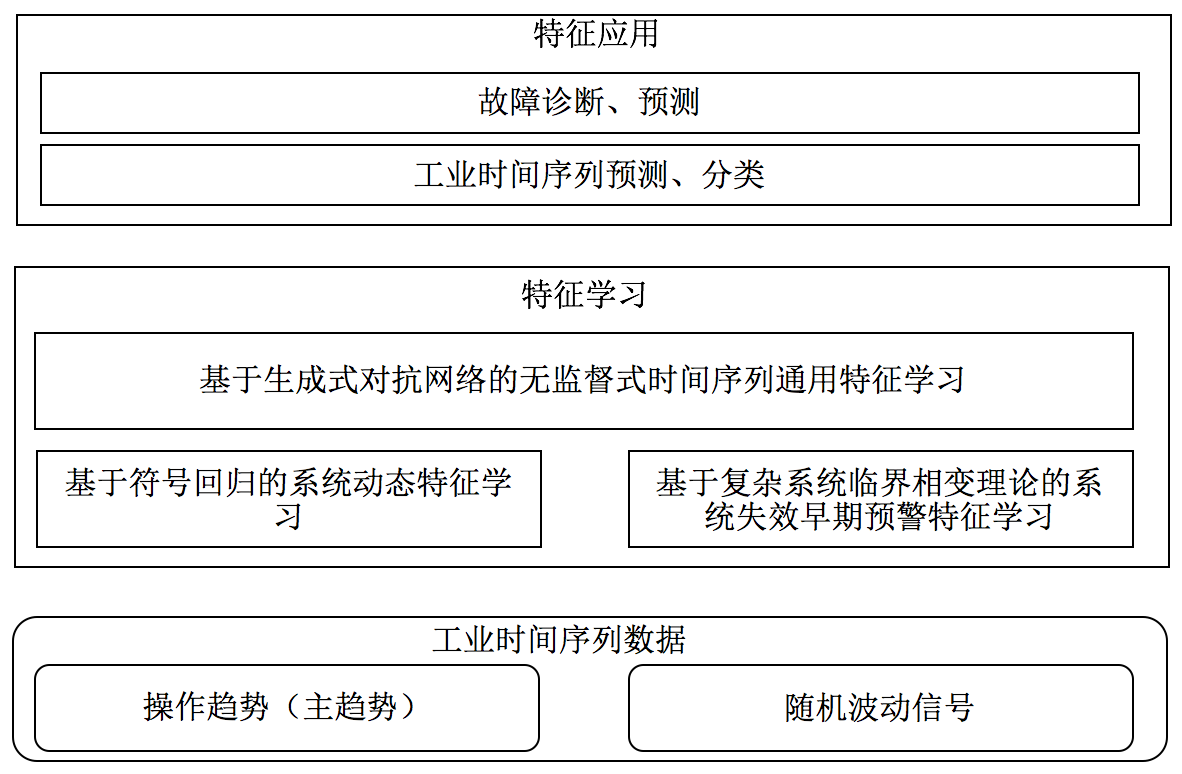
\includegraphics[scale=0.5]{figures/main-paper-framework.png}
% \caption{论文主要研究内容}
% \label{fig:paper-framework}
% \end{figure}

第 1 章:绪论
	
首先论述研究背景和意义;其次介绍本文主要研究内容和贡献。

第 2 章:相关研究综述

对相关研究,故障预测与健康管理、时间序列特征学习、非线性系统方程学习、复杂系统临界相变预测理论以及生成式对抗网络,进行梳理和综述;论述现有工作的优缺点以及与本文工作的契合点。

第 3 章:基于符号回归的系统结构特征学习与应用

针对正常运行数据普遍蕴含系统机理信息的契机,以及现有数据驱动方法对机理认识不足的问题,本文利用以轴温为代表的设备正常状态数据展开研究。首先介绍研究背景与数据分析工作;然后提出基于符号回归的系统结构特征学习方法,并融合确定性优化算法和遗传算法完成训练。一方面,系统结构特征可反映系统的动态性和信号间的相互作用关系;另一方面,将系统结构特征作为系统运行时的健康基线,设计在线实时异常检测框架。

第 4 章:基于临界相变理论的早期预警特征学习与应用

针对故障数据普遍存在小样本、不完备特性的挑战,以及现有方法普适性较差的问题,本文利用4个不同类型的系统全生命周期数据集展开研究。首先介绍研究背景并论述复杂系统临界相变预测理论对工业系统的适用性。然后提出基于复杂系统临界相变理论的早期预警特征学习方法:(1)设计随机波动信号挖掘框架,挖掘系统的固有随机波动信号;(2)基于随机波动信号学习系统失效早期预警特征,并进行有效性和鲁棒性检验;(3)基于原生时间序列,通过威尔科克森检验、核密度估计、基于AIC的ARIMA模型分析以及动态系统稳定性分析,检验假设——“系统失效与临界相变一致”。最后针对早期预警特征提出关键跳变检测算法实现故障预测。

第 5 章:基于生成式对抗网络的无监督式特征学习与应用

针对标记数据采集难、人工标记数据难的挑战,以及监督式学习方法的不足,本文利用最大的时间序列分类数据集(85个数据集)展开研究。首先简要介绍研究背景,神经网络和卷积神经网络;然后基于生成式对抗网络提出时间序列无监督式特征学习模型——时间序列生成式对抗网络 (TSGAN),并完成训练。一方面,TSGAN的生成器学习真实时间序列数据集的分布,可作为模拟器使用;另一方面,将TSGAN的判别器作为特征转换器与K近邻、支持向量机和逻辑斯蒂回归分类器结合,构建半监督式时间序列分类框架。

第 6 章:总结与展望

对本文工作以及相关结论进行概要总结;对未来工作进行展望。
% 本文的研究对于深入理解复杂工业系统运行机理,发现并预测潜在故障隐患,建立依靠先 进技术支撑的维修体制,具有重大意义。

\subsection{研究贡献}

1.本文直接基于以轴温为代表的设备正常状态数据,提出基于符号回归的系统动结构征学习方法以揭示系统机理,进一步将系统结构特征作为系统运行时的健康基线设计在线实时异常检测框架,在一定程度上弥补了现有建模方法的不足。

2.本文提出基于复杂系统临界相变理论的早期预警特征学习方法,进一步基于此提出关键跳变检测算法实现故障预测,并采用4个不同类型的数据集验证了方法有效性和通用性。此发现为针对少量失效敏感的时间序列信号设计通用的故障预测方法提供了新思路,为复杂系统临界相变预测理论的研究提供了补充。

3.本文提出无监督式时间序列特征学习通用模型——时间序列生成式对抗网络(TSGAN),进一步基于此设计半监督式时间序列分类框架,并采用最大的时间序列分类数据集(85个数据集)验证了方法的有效性。TSGAN为无监督式时间序列特征学习以及基于此的半监督式机器学习提供了新思路,丰富了GAN在时间序列领域的应用。

4.本文所有方法均得到了真实场景数据或公开数据的验证,具有较好的应用价值和借鉴意义。


